\chapter{CONCEPTION ET ÉTUDE TECHNIQUE}
	\section{Conception}
	
	Face à leur grandeur, le développement des systèmes d'information devient de plus en plus complexe. Prévoir les fonctionnalités d'un système d'information devient alors moins de en moins évidentes, c'est ainsi qu'entre en jeu la phase de conception. La phase de conception nécessite des outils permettant de mettre en place un modèle sur lequel on va s'appuyer pour réaliser notre application.
	

	\section{Présentation de UML}
			UML est un langage de modélisation très complet, qui couvre de nombreux aspects du développement des logiciels, comme les exigences, l’architecture, les structures et les comportements.\\
			
			Depuis sa normalisation, en 1997, UML a fortement évolué, passant d’un langage peu formel, principalement destiné à la documentation, à un langage suffisamment précis pour que des applications puissent être générées à partir des modèles. Cette évolution	vers une plus grande précision a cependant créé une césure entre les tenants du « tout modèle », qui demandent toujours plus de formalisme, et les développeurs, qui apprécient UML pour sa capacité à capturer en quelques dessins les grandes lignes d’une
			application.
		\subsection{Principaux diagrammes UML}
			UML dispose à sa version actuelle (2.5.1) de treize diagrammes qui sont regroupés en deux grandes catégories tels que les diagrammes structurels et les diagrammes de comportements.
		\subsubsection{Diagramme structurels}
			Ces diagrammes permettent de visualiser, spécifier, construire et documenter l'aspect statique ou structurel du système d'information. Voici quelques diagrammes utilisés couramment:\\
			\begin{itemize}
				\item Diagramme de classe: Ce diagramme représente la description statique du système en intégrant dans chaque classe la partie dédiée aux données et celle consacrée aux traitements. C’est le diagramme pivot de l’ensemble de la modélisation d’un système.\cite{definition_diagramme_classe}\\
				
				\item Diagramme de composant: Ce diagramme représente
				les différents constituants du logiciel au niveau de l’implémentation d’n système.\cite{definition_diagramme_composant}\\
				
				\item Diagramme de paquetage: Ce diagramme donne une
				vue d’ensemble du système structuré en paquetage. Chaque paquetage représente un ensemble homogène d’éléments du système (classes, composants…).\cite{definition_diagramme_paquetage}\\
			\end{itemize}
		\subsubsection{Diagramme de comportements}
			Les diagrammes comportementaux modélisent les aspects dynamiques du système, c'est à dire les différents éléments qui sont susceptibles de subir des modifications.\\
		\subsection{Diagramme de cas d'utilisation}
		Un cas d'utilisation est une unité cohérente représentant une fonctionnalité visible de l'extérieur. Un cas d'utilisation modélise donc un service rendu par le système.\cite{cas_d_utilisation}\\
		\\Implémentation:\\
		\subsubsection{Acteurs:}
			\begin{itemize}
				\item[$\bullet$] \textbf{Administrateur} : Acteur ayant pour rôle de gérer les comptes des autres utilisateurs de l'application.\\
				\item[$\bullet$]  \textbf{Agent(Personnel)} : Agent de l'entreprise ayant accès à l'application depuis un point de vente agrée.\\
				\item[$\bullet$] \textbf{Validateur}: système externe qui récupère les messages des opérations effectuées et les valide par USSD. Le validateur peut être une application mobile ou un autre système.\\
			\end{itemize}
		\subsubsection{Identification des cas d’utilisation:}
			\begin{itemize}
				\item[$\bullet$]  \textbf{Authentification}
				\item[$\bullet$] \textbf{Gestion des comptes}
				\item[$\bullet$] \textbf{Gestion des intermèdes}
				\item[$\bullet$] \textbf{Gestion des numéros}
				\item[$\bullet$] \textbf{Gestion des opération}
				\item[$\bullet$] \textbf{Gestion des messages}
			\end{itemize}
		\subsubsection{Implémentation}
			\begin{center}
				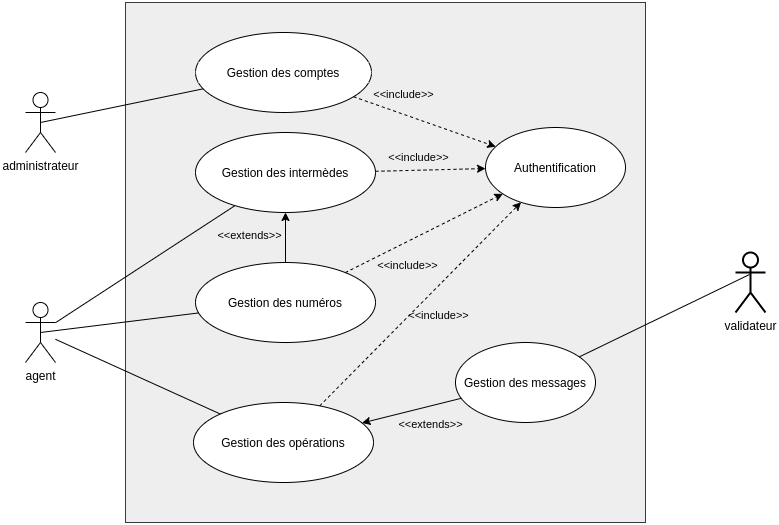
\includegraphics[width=16cm]{chap_2/use-case.png}
				\captionof{figure}{Diagramme de cas d'utilisation : vue globale}
				\label{figure9}
			\end{center}
		\subsubsection{Étude détaillée des cas d'utilisation}
		\newpage
		\subsection*{Authentification}
			 \begin{table}[!h]
			 	\begin{center}
			 		\noindent {\renewcommand{\arraystretch}{1.5}\begin{tabularx}{\textwidth}{|l|X|}
			 				\hline & Description \\
			 				\hline Acteur principal & Agent de l'entreprise \\
			 				\hline Objectif & Se connecter pour avoir accès aux différentes fonctionnalités de l'application\\
			 				\hline Pré-conditions & Les informations sur l'agent doivent exister dans la base de données.\\
			 				\hline Déclencheur & Lancement de la page d'authentification\\
			 				\hline
			 				Scénario nominal & Affichage du formulaire de connexion contenant l'email et le mot de passe. 
			 				L'agent renseigne ses identifiants et le système à son tour vérifie l'authenticité de ces informations.\newline
			 				Si ces informations sont correctes alors l'agent est dirigé vers la page d'accueille.
			 				\\
			 				\hline
			 				Extensions &  Si les identifiants envoyés sont incorrectes alors un message d'erreur lui est envoyé. \\ 
			 				\hline               
			 		\end{tabularx}}
			 	\end{center}
			 	\caption{Description de l'authentification} 
			 	\label{Tableau authentification}
			 \end{table}
			 \noindent
		\newpage
		\subsection*{Gestion des comptes}
		Dans cas d'utilisation, il revient à l'administrateur du système de créer les comptes des différents agents du système et leur attribuer un rôle à certaines pages de l'application en fonction de leurs rôles.
			\begin{center}
				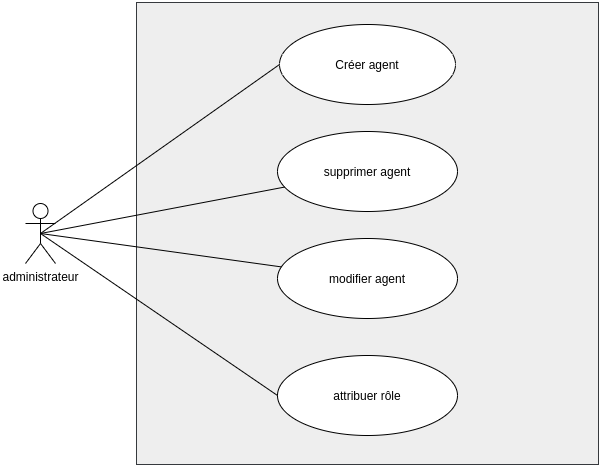
\includegraphics[scale=0.5]{chap_2/gestion-compte.png}
				\captionof{figure}{Diagramme de cas d'utilisation : gestion des comptes}
				\label{cas d'utilisateur gestion compte}
			\end{center}
			\begin{table}[H]
				\begin{center}
					 {\renewcommand{\arraystretch}{1.5}\begin{tabularx}{\textwidth}{|l|X|}
							\hline & Description \\
							\hline Acteur principal & Administrateur\\
							\hline Objectif & Enregistrer les agents de l'entreprise dans la base de donnée et attribuer à chacun d'eux un rôle.\\
							\hline Pré-conditions & Etre authentifier et avoir le rôle \textbf{admin}\\
							\hline Déclencheur & Lancement de la page d'authentification\\
							\hline
							Scénario nominal & Affichage du formulaire de connexion contenant l'email et le mot de passe. 
							L'utilisateur saisit ses identifiants et le système à son tour vérifie l'authenticité de des données entrées.\newline
							Si les informations entrées sont correctes alors l'agent est dirigé vers la page d'administration.
							\\
							\hline
							Extensions &  Si les informations entrées sont incorrectes alors un message d'erreur lui est envoyé. \\
							\hline               
					\end{tabularx}}
				\end{center}
				\caption{Description de cas d'utilisation : Gestion des compte} 
				\label{Table compte}
			\end{table}
		\subsection*{Gestion des intermèdes}
			Dans ce cas d'utilisateur, la tâche revient au personnel agent de gérer tout ce qui concerne les intermèdes.
			\begin{center}
				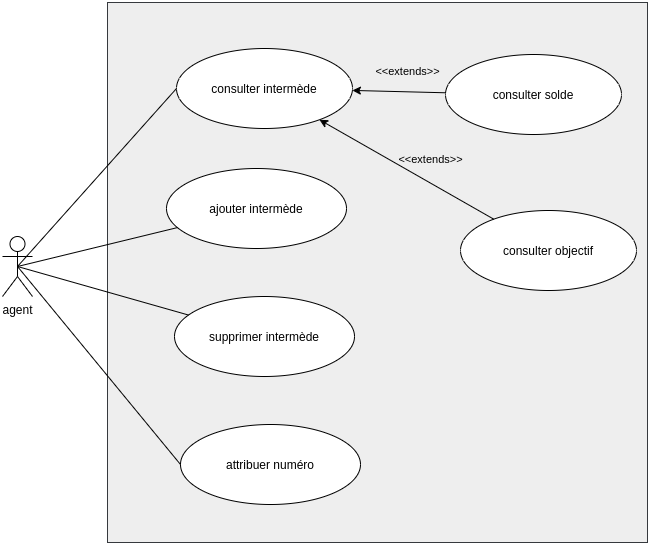
\includegraphics[scale=0.5]{chap_2/use-intermede.png}
				\captionof{figure}{Diagramme de cas d'utilisation : gestion des comptes}
				\label{cas d'utilisateur gestion des intermèdes}
			\end{center}
			\begin{table}[!h]
				\begin{center}
					{\renewcommand{\arraystretch}{1.5}\begin{tabularx}{\textwidth}{|l|X|}
							\hline & Description \\
							\hline Acteur principal & Agent de l'entreprise \\
							\hline Objectif & Avoir la possibilité de gérer la liste des intermèdes dans le but de pouvoir l'étendre, réduire et mettre à jour des informations les concernant .\\
							\hline Pré-conditions & Être authentifié\\
							\hline Description & Une fois l'agent connecté, il a accès aux différentes pages qui lui permettront de gérer les intermèdes
							\\
							\hline              
					\end{tabularx}}
				\end{center}
				\caption{Description du cas d'utilisation: Gestion des intermèdes}
			\end{table}
		\subsection*{Gestion des numéros}
			\begin{table}[H]
				\begin{center}
					{\renewcommand{\arraystretch}{1.5}\begin{tabularx}{\textwidth}{|l|X|}
							\hline & Description \\
							\hline Acteur principal & Agent de l'entreprise \\
							\hline Objectif & Mettre à jour les numéros des intermèdes, créer de nouveaux numéros.\\
							\hline Pré-conditions & Avoir au moins un intermède existant.\\
							\hline Déclencheur & Lancement de la page d'authentification.\\
							\hline
							Scénario nominal &
							Choisir l'intermède.\newline
							Saisir le numéro.\newline
							Attribuer numéro.\newline\newline
							Enregistrer un numéro.\newline
							Mettre à jour numéro.\newline
							Supprimer numéro.\\
							\hline
							Extensions & Si aucun intermède n'existe alors il sera impossible d'enregistrer un nouveau numéro. \\ 
							\hline               
					\end{tabularx}}
				\end{center}
				\caption{Description du cas d'utilisateur : Gestion des numéros}
			\end{table}
		\subsection*{Gestion des opérations}
			\begin{center}
				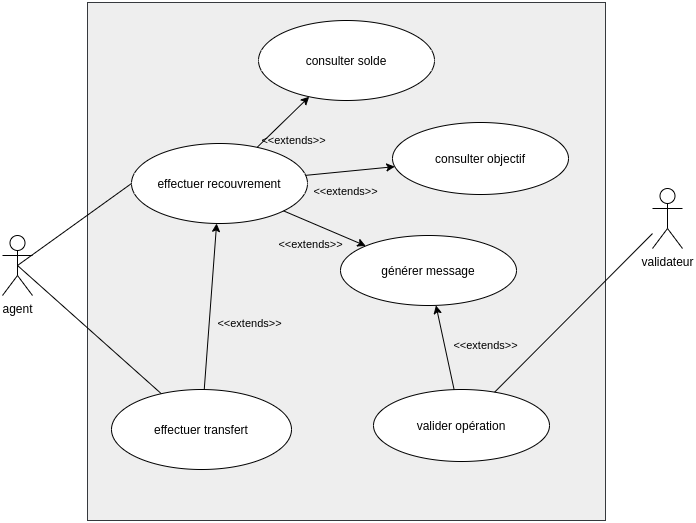
\includegraphics[scale=0.5]{chap_2/gestion-operation.png}
				\captionof{figure}{Diagramme de cas d'utilisation : gestion des opérations}
				\label{Gestion des opérations}
			\end{center}
			\begin{table}[H]
				\begin{center}
					{\renewcommand{\arraystretch}{1.5}\begin{tabularx}{\textwidth}{|l|X|}
							\hline & Description \\
							\hline Acteur principal & Agent de l'entreprise et validateur \\
							\hline Objectif & Effectuer recouvrement(Dépôt ) et transfert d'argent sur les numéros des intermèdes\\
							\hline Pré-conditions & Être authentifié\\
							\hline
							Scénario nominal & Sélectionner le grâce à son code ou son nom.\newline
							Saisir le montant à transférer.\newline\newline
							Choisir le mode de paiement. Si le mode de paiement choisit correspond à un paiement bancaire, alors un nouveau champ apparait pour saisir la référence bancaire. Dans le cas d'un recouvrement ou dépôt tous les modes de paiement de paiement sont autorisés sauf le mode de paiement à crédit.\newline\newline
							Lancer l'opération.\newline\newline
							Un message approuvant le qui l'opération a été effectuée est généré.\newline\newline
							Le validateur récupère le message et valide le opération de manière concrète grâce à la syntaxe appropriée par exemple il effectue:\newline
							*413*NUMERO*MONTANT*00000\# sachant bien que le NUMERO et le MONTANT sont contenus dans le message récupéré.\newline
							Une fois l'opération validée concrètement, le validateur renvoie reçu.\newline
							Impression de la facture.
							\\
							\hline
							Extensions &  Si les informations envoyées sont incorrectes alors un message d'erreur est affiché \\ 
							\hline               
					\end{tabularx}}
				\end{center}
				\caption{Description du cas d'utilisateur : Gestion des opérations}
			\end{table}
		\subsection*{Gestion des messages}
			\begin{center}
				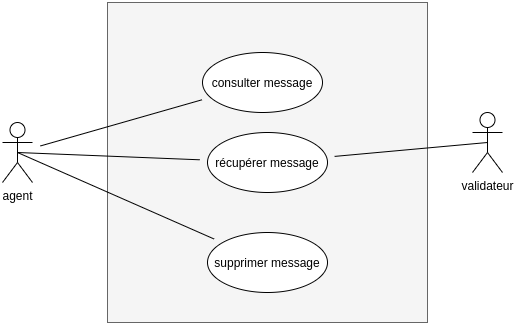
\includegraphics[scale=0.5]{chap_2/message.png}
				\captionof{figure}{Diagramme de cas d'utilisation : gestion des messages}
				\label{Gestion des messages}
			\end{center}
			\begin{table}[H]
				\begin{center}
					{\renewcommand{\arraystretch}{1.5}\begin{tabularx}{\textwidth}{|l|X|}
							\hline & Description \\
							\hline Acteur principal & Agent et validateur \\
							\hline Objectif & Traiter les messages générés après chaque opération.\\
							\hline Pré-conditions & . Être authentifié\\
							\hline Déclencheur & Opération effectuée\\
							\hline
							Scénario nominal & Une fois qu'une opération est effectuée, un  nouveau message est généré avec \textbf{l'état initié}.\newline
							Une fois que le message est récupéré, son état du message passe à l'état '\textbf{en cours d'exécution}'.\newline
							Enfin, lorsque l'opération est finalement validée, alors l'etat du message passe à \textbf{clôturer}
							\\
							\hline              
					\end{tabularx}}
				\end{center}
				\caption{Description de l'authentification} 
			\end{table}
		\subsection{Diagramme de classe}
			\subsubsection{Définition de classe}
				Une classe est un ensemble de données et de fonctions regroupées dans une même entité. Une classe est une description abstraite d'un objet. Les fonctions permettant de manipuler la classe sont appelées méthodes. Instancier une classe consiste à créer un objet sur son modèle.
			\subsubsection{Représentation d'une classe}
				Une classe est représentée par rectangle subdiviser en trois compartiments dans laquelle:
				\begin{itemize}
					\item Le premier compartiment contient le nom de classe
					\item Le deuxième contient la liste des attributs de classe ainsi que leur visibilité (public, protégée ou privée).
					\item Le troisième compartiment représente la liste des méthodes permettant de manipuler les différents attributs de classe.
				\end{itemize}
			En gros une classe se présente comme le montre la figure suivante:
			\begin{center}
				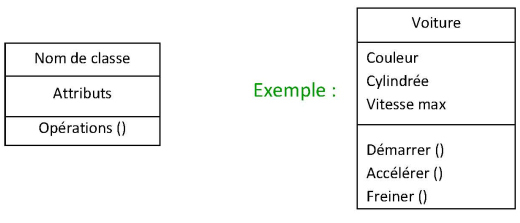
\includegraphics{images/img-1.jpg}\cite{image_classe_voiture}
				\captionof{figure}{représentation d'une classe}
				\label{figure1}
			\end{center}
			\subsubsection{Les attributs}
				Les attributs représentent les données qui caractérisent l'objet. Les attributs sont aussi définis par leurs types (entier, chaîne de caractère, caractère, etc. ).
			\subsubsection{Les méthodes}
				Les méthodes d'un objet caractérisent son comportement, c'est-à-dire l'ensemble des actions (appelées opérations) que l'objet est à même de réaliser.
			\subsubsection{Notion de multiplicité}
				La multiplicité définit le nombre d'instances de l'association pour une instance de la classe.
				La multiplicité est définie par un nombre entier ou un intervalle de valeurs, elle est aussi la traduction d'une règle de gestion.
				\begin{center}
					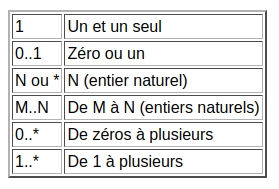
\includegraphics{images/img-2.png}
					\captionof{figure}{multiplicité}
					\label{figure2}
				\end{center}
			\subsubsection{Les associations}
			Les associations permettent de préciser les relations qui peuvent exister entre deux ou plusieurs objets.
			L'association se fait entre classe et non entre les instances. Lorsqu'une association est
			définie entre deux classes, cela signifie que les objets instances de ces deux classes
			peuvent être reliés entre eux.
			\begin{center}
				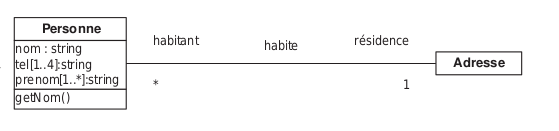
\includegraphics[width=\columnwidth]{images/assoc-1.png}
				\captionof{figure}{association}
				\label{figure3}
			\end{center}
		\subsubsection{implémentation}
		Identification des classes:\\
		
		\textbf{Personnel}(ID:integer, nom:string, prenom:string, email)\\
		
		\textbf{Intermed}(ID:integer, code:string, nom:string, solde:integer)\\
		
		\textbf{Numero}(ID:integer, numero:string)\\
		
		\textbf{Objectif}(ID:integer, mois:string, objectif:integer, bilan:integer)\\
		
		\textbf{Operation}(ID:integer, montant:integer, reference:string, date)\\
		
		\textbf{Transfert}(ID:integer, numero:string)\\
		
		\textbf{Secteur}(ID:integer, nom:string)\\
		
		\textbf{Agence}(ID:integer, nom:string)\\
		
		\textbf{Statut}(ID:integer, nom:string)\\
		
		\textbf{Etat}(ID:integer, nom:string, commentaire:text)\\
		
		\textbf{Message}(ID:integer, sms:text, date:Date)\\
		
		\textbf{Facture}(ID:integer, numeroFac:string, date:Date)\\
		
		\textbf{Mode de paiement}(ID:integer, nom:string)\\
		
		\textbf{Ouverture}(ID:integer, jour:string, code:string)\\
		
		\begin{center}
			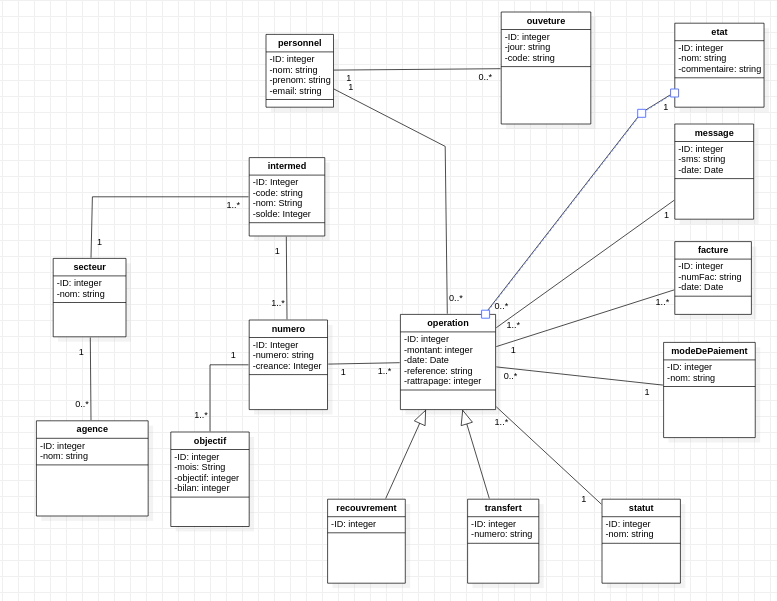
\includegraphics[width=16cm]{images/diagramme.png}
			\captionof{figure}{diagramme de classe de l'application}
		\end{center}
	
	\subsubsection{Description des classe}
	
		\begin{center}
			{\renewcommand{\arraystretch}{1.5}\begin{tabularx}{\textwidth}{|l|l|l|X|}
				\hline
				\multicolumn{4}{|c|}{\textbf{Classe Peronnel : représente les effectuant les opérations}}\\
				\hline
				
				& \textbf{Nom} & \textbf{Description} & \textbf{Type} \\
				\multirow{4}{*}{Attributs} & ID & code permettant d'identifié le personnel & Numérique \\
				& nom & désigne le nom personnel & chaîne de caractère \\
				& prénom & désigne le prénom de personnel & chaîne de caractère \\
				& email & addresse électronique de l'intermed & chaîne de caractère\\
				\hline
			\end{tabularx}}
			\captionof{table}{tableau de classe \textit{Personnel}}
			\label{classe personnel}
		\end{center}
	
		\begin{center}
			{\renewcommand{\arraystretch}{1.5}\begin{tabularx}{\textwidth}{|l|l|l|X|}
					\hline
					\multicolumn{4}{|c|}{\textbf{Classe Intermed : représente les effectuant les opérations}} \\
					
					\hline
					
					& \textbf{Nom} & \textbf{Description} & \textbf{Type} \\
					\multirow{3}{*}{Attributs} & ID & code permettant d'identifié l'intermed & numérique \\
					
					& code & code unique permettant d'identifier l'intermed &  chaîne de caractère \\
					
					& nom & désigne le nom l'intermède & chaîne de caractère \\
					
					& solde & désigne le solde l'intermède & numérique \\
					\hline
			\end{tabularx}}
			\captionof{table}{tableau de classe Intermed}
			\label{classe intermède}
		\end{center}
	
		\begin{center}
			{\renewcommand{\arraystretch}{1.5}\begin{tabularx}{\textwidth}{|l|l|l|X|}
					\hline
					\multicolumn{4}{|c|}{\textbf{Classe Numéro : numéro appartenant à un intermède}} \\
					
					\hline
					
					& \textbf{Nom} & \textbf{Description} & \textbf{Type} \\
					\multirow{3}{*}{Attributs} & ID & permet d'identifier le numéro & numérique \\
					
					& numéro & numéro de l'intermède & chaîne de caractère \\
					
					& créance & créance de l'intermède sur ce numéro  & numérique \\
					
					\hline
			\end{tabularx}}
			\captionof{table}{tableau de classe \textit{Numéro}}
			\label{classe numero}
		\end{center}
		
		
		\begin{center}
			{\renewcommand{\arraystretch}{1.5}\begin{tabularx}{\textwidth}{|l|l|l|X|}
					\hline
					\multicolumn{4}{|c|}{\textbf{Classe Objectif : représente les effectuant les opérations}} \\
					
					\hline
					
					& \textbf{Nom} & \textbf{Description} & \textbf{Type} \\
					\multirow{3}{*}{Attributs} & ID & identifiant de l'objectif d'un numéro & numérique \\
					
					& mois & mois dans lequel l'objectif à été effectué &  chaîne de caractère \\
					
					& objectif & objectif du numéro &chaîne de caractère \\
					
					& bilan & bilan de l'objectif & numérique \\
					
					\hline
			\end{tabularx}}
			\captionof{table}{tableau de classe \textit{objectif}}
			\label{classe objectif}
		\end{center}
	
		\begin{center}
		%	\noindent\setlength\tabcolsep{1pt}%
			{\renewcommand{\arraystretch}{2}\begin{tabularx}{\textwidth}{|l|l|p{0.5\linewidth}|X|}
					\hline
					\multicolumn{4}{|c|}{\textbf{Classe Opération: désigne les opérations pouvant être par le personnel}} \\
					
					\hline
					
					& \textbf{Nom} & \textbf{Description} & \textbf{Type} \\
					\multirow{3}{*}{Attributs} & ID & identifiant de l'opération & numérique \\
					
					& montant & montant à transféré ou à déposer & numérique\\
					
					& date & date à laquelle l'opération s'est effectuée & numérique \\
					
					& référence & chaîne de caractère pouvant identifier l'opération & chaîne de caractère\\
					
					& rattrapage & entier permettant de spécifier si l'opération s'est bien déroulée & entier \\
					
					\hline
			\end{tabularx}}
			\captionof{table}{tableau de classe \textit{Opération}}
			\label{table5}
		\end{center}
		
		
		\begin{center}
			\noindent
			{\renewcommand{\arraystretch}{2}\begin{tabularx}{\linewidth}{|l|l|p{0.5\linewidth}|X|}
					\hline
					\multicolumn{4}{|c|}{\textbf{Classe État : définie l'ensemble des statut que peux pendre une opération}} \\
					
					\hline
					
					& \textbf{Nom} & \textbf{Description} & \textbf{Type} \\
					\multirow{3}{*}{Attributs} & ID & code permettant d'identifié l'intermède & numérique \\
					
					& nom & nom du statut qui peut prendre les valeurs suivantes: \textit{initié},
					\textit{en cours d'exécution}, \textit{exécuté}, \textit{annulé} et \textit{supprimé} & chaine de caractère\\
					
					\hline
			\end{tabularx}}
			\captionof{table}{tableau de classe \textit{Opération}}
			\label{classe Etat}
		\end{center}
	
		\begin{center}
			{\renewcommand{\arraystretch}{1.5}\begin{tabularx}{\textwidth}{|l|l|l|X|}
					\hline
					\multicolumn{4}{|c|}{\textbf{Classe Message : message de transfert après qu'une opération soit effectuée}} \\
					
					\hline
					
					& \textbf{Nom} & \textbf{Description} & \textbf{Type} \\
					\multirow{3}{*}{Attributs} & ID & identifiant du message & numérique \\
					
					& sms & message de transfert &  texte\\
					
					& date & date à laquelle le message a été reçu & date \\
					
					\hline
			\end{tabularx}}
			\captionof{table}{tableau de classe \textit{message}}
			\label{table7}
		\end{center}
		
		
		\begin{center}
			{\renewcommand{\arraystretch}{1.5}\begin{tabularx}{\textwidth}{|l|l|l|X|}
					\hline
					\multicolumn{4}{|c|}{\textbf{Classe transfert : classe fille de la classe opération spécialisée dans le transfert}} \\
					
					\hline
					
					& \textbf{Nom} & \textbf{Description} & \textbf{Type} \\
					\multirow{3}{*}{Attributs} & ID & permet d'identifier le transfert effectué & numérique \\
					
					& numéro & numéro sur lequel le transfert sera effectué & chaîne de caractère\\
					
					\hline
			\end{tabularx}}
			\captionof{table}{tableau de classe \textit{transfert}}
			\label{table15}
		\end{center}
		
	%--------------------------------------------------------------------
		
		\begin{center}
			{\renewcommand{\arraystretch}{1.5}\begin{tabularx}{\textwidth}{|l|l|l|X|}
				\hline
				\multicolumn{4}{|c|}{\textbf{Classe recouvrement : classe spécialisée dans le recouvrement}} \\
				
				\hline
				
				& \textbf{Nom} & \textbf{Description} & \textbf{Type} \\
				\multirow{1}{*}{Attributs} & ID & permet d'identifier le recouvrement effectué & numérique \\
				\hline
			\end{tabularx}}
			\captionof{table}{tableau de classe \textit{recouvrement}}
			\label{table16}
		\end{center}
	%-----------------------------------------------------------------------------
		
		
			\begin{center}
			{\renewcommand{\arraystretch}{1.5}\begin{tabularx}{\textwidth}{|l|l|l|X|}
					\hline
					\multicolumn{4}{|c|}{\textbf{Classe Facture : facture délivrée après une opération}} \\
					\hline
					
					& \textbf{Nom} & \textbf{Description} & \textbf{Type} \\
					\multirow{3}{*}{Attributs} & ID & identifiant permettant de retrouver la facture & numérique \\
					
					& numFac & numéro unique permettant d'identifier la facture &  chaîne de caractère \\
					
					& date & date à laquelle la facture a été délivrée & chaîne de caractère \\
					
					\hline
			\end{tabularx}}
			\captionof{table}{tableau de classe \textit{facture}}
			\label{table8}
		\end{center}
		%-----------------------------------------------------------------------------
		
		\begin{center}
			{\renewcommand{\arraystretch}{1.5}\begin{tabularx}{\textwidth}{|l|l|l|X|}
					\hline
					\multicolumn{4}{|c|}{\textbf{Classe ModePaiement : représente les effectuant les opérations}} \\
					
					\hline
					
					& \textbf{Nom} & \textbf{Description} & \textbf{Type} \\
					\multirow{3}{*}{Attributs} & ID & identifiant unique attribué à un mode paiement  & numérique \\
					
					& nom & nom du mode de paiement &  chaîne de caractère \\
					
					\hline
			\end{tabularx}}
			\captionof{table}{tableau de classe \textit{ModePaiement}}
			\label{table9}
		\end{center}
		%-----------------------------------------------------------------------------
		
		\begin{center}
			{\renewcommand{\arraystretch}{1.5}\begin{tabularx}{\textwidth}{|l|l|l|X|}
					\hline
					\multicolumn{4}{|c|}{\textbf{Classe ouverture : représente les effectuant les opérations}} \\
					
					\hline
					
					& \textbf{Nom} & \textbf{Description} & \textbf{Type} \\
					\multirow{3}{*}{Attributs} & ID & identifiant des jours d'ouverture & numérique \\
					
					& jour & jour d'ouverture & chaîne de caractère \\
					
					& code & code d'ouverture & chaîne de caractère \\
					\hline
			\end{tabularx}}
			\captionof{table}{tableau de classe \textit{ouverture}}
			\label{table10}
		\end{center}
		%-----------------------------------------------------------------------------
		
		
		\begin{center}
			{\renewcommand{\arraystretch}{1.5}\begin{tabularx}{\textwidth}{|l|l|l|X|}
				\hline
				\multicolumn{4}{|c|}{\textbf{Classe agence : définie l'agence}} \\
				
				\hline
				
				& \textbf{Nom} & \textbf{Description} & \textbf{Type} \\
				\multirow{3}{*}{Attributs} & ID & identifiant permettant d'identifier l'agence & numérique \\
				
				& nom & désigne le nom de l'agence& chaîne de caractère \\
				
				\hline
			\end{tabularx}}
			\captionof{table}{tableau de classe \textit{agence}}
			\label{table14}
		\end{center}
		%-----------------------------------------------------------------------------
		
		
		\begin{center}
			{\renewcommand{\arraystretch}{1.5}\begin{tabularx}{\textwidth}{|l|l|l|X|}
					\hline
					\multicolumn{4}{|c|}{\textbf{Classe Secteur : secteur au lequel appartient l'agence}} \\
					
					\hline
					
					& \textbf{Nom} & \textbf{Description} & \textbf{Type} \\
					\multirow{3}{*}{Attributs} & ID & identifiant du secteur & numérique \\
					
					& nom & nom du secteur &  chaîne de caractère \\
					
					\hline
			\end{tabularx}}
			\captionof{table}{tableau de classe \textit{secteur}}
			\label{table11}
		\end{center}
		%-----------------------------------------------------------------------------
		
		
		\section{Schéma relationnel}
			\subsection{Modèle logique des données ou MLD}
				\subsubsection{Définition}
					Le modèle logique des données consiste à décrire la structure de données utilisée sans faire référence à un langage de programmation. Il s'agit donc de préciser le type de données utilisées lors des traitements. Ainsi, le modèle logique est dépendant du type de base de données utilisé.
				\subsubsection{Liste des tables}
					
					\textbf{PERSONNEL}(\underline{\textbf{ID}}, nom, prenom, email)\\
					
					\textbf{SECTEUR}(\underline{\textbf{ID}}, nom)\\
					
					\textbf{AGENCE}(\underline{\textbf{ID}}, \#secteur\_id, nom)\\
					
					\textbf{INTERMED}(\underline{\textbf{ID}}, code, nom, solde)\\
					
					
					\textbf{NUMERO}(\underline{\textbf{ID}}, \#intermed\_id, numero, creance)\\
					
					\textbf{objectif}(\underline{\textbf{ID}}, \#numero\_id, mois, objectif, bilan)\\
					
					\textbf{MODEDEPAIEMENT}(\underline{\textbf{ID}}, nom)\\
					
					\textbf{STATUT}(\underline{\textbf{ID}}, nom)\\
					
					\textbf{ETAT}(\underline{\textbf{ID}}, nom)\\
					
					\textbf{OPERATION}(\underline{\textbf{ID}}, \#personnel\_id, \#numero\_id, \#modepaiement\_id, \#statut\_id, \#etat\_id, montant, date, reference, rattrapage)\\
					
					\textbf{OUVERTURE}(\underline{\textbf{ID}}, \#personnel\_id, jour, code)\\
					
					\textbf{TRANSFERT}(\underline{\textbf{ID}},\#personnel\_id, \#numero\_id, \#modepaiement\_id, \#statut\_id, \#etat\_id, rattrapage, montant, reference, date)\\
					
					\textbf{RECOUVREMENT}(\underline{\textbf{ID}},\#personnel\_id, \#modepaiement\_id, \#statut\_id, \#etat\_id, rattrapage, montant, reference, date)\\
					
					\textbf{FACTURE}(\underline{\textbf{ID}}, \#operation\_id, numFac, date)\\
					
					\textbf{MESSAGE}(\underline{\textbf{ID}}, \#operation\_id, sms, date)\\
			\subsection{Modèle physique de donnée ou MPD}
			
				\subsubsection{Définition}
					Un modèle de données physique est un modèle spécifique à une base de données, qui représente des objets de données relationnelles (par exemple, tables, colonnes, clés principales et externes) et leurs relations.
				\subsubsection{Représentation du MPD}
					\includegraphics[width=\columnwidth]{images/database.png}
					\captionof{figure}{Modèle physique des données}
					\label{modèle physique des données}
	\section{Outils de développement}
		\subsection{Technologie front-end}
			\subsubsection{HTML 5}
				L'HyperText Markup Language, HTML, désigne un type de langage informatique descriptif. Il s'agit plus précisément d'un format de données utilisé dans l'univers d'Internet pour la mise en forme des pages Web. Il permet, entre autres, d'écrire de l'hypertexte, mais aussi d'introduire des ressources multimédias dans un contenu.\\
				
				Développé par le W3C (World Wide Web Consortium) et le WHATWG (Web Hypertext Application Technology Working Group), le format ou langage HTML est apparu dans les années 1990. Il a progressivement subi des modifications et propose depuis 2014 une version HTML5 plus aboutie.\\
				
				L'HTML est ce qui permet à un créateur de sites Web de gérer la manière dont le contenu de ses pages Web va s'afficher sur un écran, via le navigateur.\cite{definition_html}
				
				\begin{center}
					
\includegraphics[width=2cm]{chap_2/html5.png}
					\captionof{figure}{Logo HTML 5}
					\label{figure5}
				\end{center}
			
			\subsubsection{CSS 3}
			
			Les feuilles de styles (en anglais "Cascading Style Sheets", abrégé CSS) sont un langage qui permet de gérer la présentation d'une page Web. Le langage CSS est une recommandation du World Wide Web Consortium (W3C), au même titre que HTML ou XML. Aujourd'hui nous sommes à la version 3 d'où CSS 3.
				
				\begin{center}
					
\includegraphics[width=2cm]{chap_2/css3.png}
					\captionof{figure}{Logo CSS 3}
					\label{figure6}
				\end{center}
			
			\subsubsection{Bibliothèque CSS - Bootstrap 5}
				
				Bootstrap est une bibliothèque CSS permettant de donner une apparence sublime aux sites web.L'une de ces forces est son côté responsive qui permet au site de s'adapter sur les grands et petits écrans (mobile)
				
				\begin{center}
					
\includegraphics[width=5cm]{chap_2/bootstrap.png}
					\captionof{figure}{Logo Bootstrap 5}
					\label{figure7}
					\cite{logo_bootstrap}
				\end{center}
			
			\subsubsection{Bibliothèque  JavaScript - AlpineJS}
			
			Alpine est un outil robuste et minimal pour composer des comportements directement dans notre code HTML. Il apporte une réactive flexible comme d'autre bibliothèque JS (React par exemple).\\
		
			\begin{center}
				
\includegraphics[width=10cm]{chap_2/alpine.png}
				\captionof{figure}{Logo AlpineJS}
				\label{figure8}
				\cite{logo_alpine}
			\end{center}
				
		\subsection{Choix du framework back-end}
			\section*{Laravel}
				\begin{center}
					
\includegraphics[scale=0.2]{chap_2/laravel.png}
					\captionof{figure}{Logo de Laravel}
					\label{logo de laravel}
					\cite{logo_laravel}
				\end{center}
			Dans cette application, nous avons décidé de nous tourner vers l'un des framework PHP le plus populaire et le plus utilisé : \textbf{Laravel}.\newline
			En effet Laravel est le framework PHP open source le mieux noté sur GitHub. Fondé en 2011 par Taylor Otwell, Laravel utilise le pattern MVC et est orienté objet.\cite{laravel_1}\newline
			Que de réinventer la roue, Laravel se base sur des technologies existantes.\\
			Laravel se base sur \textbf{Symfony} pour créer son système de routage. De même pour l'envoie des mails Laravel utilise la bibliothèque \textbf{SwiftMailer}.
			\subsection*{Avantage}
				\begin{itemize}
					\item[$\bullet$] Il est facile à installer et présent chez tous les hébergeurs.
					\item[$\bullet$] Basé sur l'architecture MVC(Model View Controller)qui donne une meilleure organisation au niveau du code et avec une hiérarchie de dossiers très bien fait.
					\item[$\bullet$] Grande communauté et beaucoup de documentation
					\item[$\bullet$] Possibilité de faire tests unitaires afin de garantir qu’il n’y a pas de bogues ou d’exceptions l'application
					\item[$\bullet$] Développement plus rapide grâce aux helpers déjà disponible.
				\end{itemize}
			\section*{Livewire}
				\begin{center}
					
\includegraphics[scale=0.6]{chap_2/livewire.png}
					\captionof{figure}{Logo de Livewire}
					\label{logo de livewire}
					\cite{logo_livewire}
				\end{center}
				\subsection*{Présentation}
					Livewire est un package Laravel, qui aux permet développeur Laravel de créer des applications Web réactives en utilisant Laravel Blade comme langage de templating sans écrit la moindre ligne de code.
					
				\subsection*{Avantages}
				\begin{itemize}
					\item[$\bullet$] Créer des application réactive en restant dans le confort Laravel sans écrit la moindre ligne de code JavaScript.
					\item[$\bullet$] Crée facilement des composants réutilisables
					\item[$\bullet$] Plusieurs fonctions (ou encore \textbf{helper}) disponible pour rendre encore plus facile sa prise en main.
				\end{itemize}
			
			
		\subsection{Système de gestion de base de données}
		\newpage
			\section*{MySQL}
			\begin{center}
				
\includegraphics[scale=0.2]{chap_2/mysql.png}
				\captionof{figure}{Logo de MySQL}
				\label{logo de MySQL}
				\cite{logo_mysql}
			\end{center}
			Et surtout MySQL, qui est un Système de Gestion de Bases de Données Relationnelles (abrégé SGBDR), c'est-à-dire un logiciel qui permet de gérer des bases de données, et donc de gérer de grosses quantités d'informations. Il utilise pour cela le langage SQL. Il s'agit d'un des SGBDR les plus connus et les plus utilisés.
			\subsection{Avantages}
				\begin{itemize}
					\item[$\bullet$] Grâce à sa popularité, MySQL dispose d'une grande communauté, ce qui implique qu'on peut facilement trouver de l'aide en cas de difficulté.
					\item[$\bullet$] il est totalement open source et gratuit.
					\item[$\bullet$] il est en plus multi-threadé et multi-utilisateurs.
					\item[$\bullet$] Ses performances sont excellentes
				\end{itemize}
			
		\subsection{Architecture structurel}
		\subsection*{MVC}
			Modèle-vue-contrôleur ou MVC est un motif d'architecture logicielle destiné aux interfaces graphiques lancé en 1978 et très populaire pour les applications web. Le motif est composé de trois types de modules ayant trois responsabilités différentes : les modèles, les vues et les contrôleurs.
				
				\begin{center}
					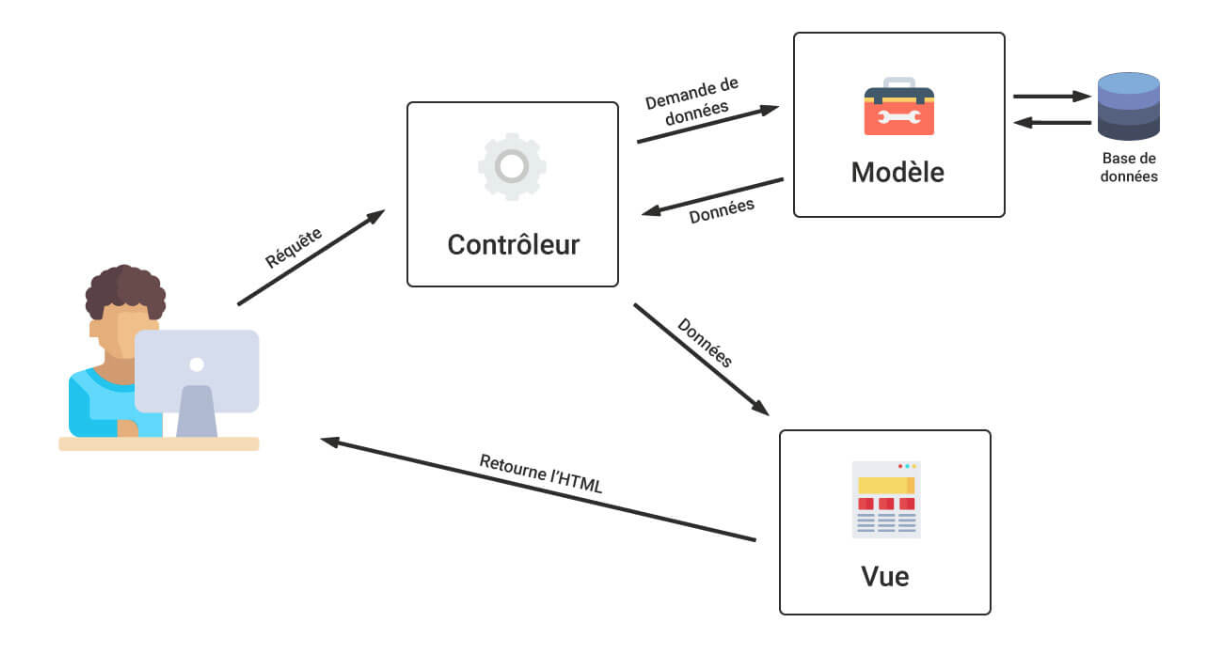
\includegraphics[scale=0.5]{chap_2/mvc.png}
					\captionof{figure}{MVC}
					\label{logo de MVC}
					\cite{logo_mvc}
				\end{center}
				
			\subsubsection{Model}
				cette partie gère les données de l'application. Son rôle est d'aller récupérer les informations « brutes » dans la base de données, de les organiser et de les assembler pour qu'elles puissent ensuite être traitées par le contrôleur. On y trouve donc entre autres les requêtes SQL\cite{mvc_model}. Dans une application laravel le Model est géré par Eloquent qui est Object Relationnal Mapping.
			\subsubsection{View}
				 Cette partie se concentre sur l'affichage. Elle ne fait presque aucun calcul et se contente de récupérer des variables pour savoir ce qu'elle doit afficher. On y trouve essentiellement du code HTML mais aussi quelques boucles et conditions PHP très simples.
			\subsubsection{Controller}
				Cette partie gère la logique du code qui prend des décisions. C'est en quelque sorte l'intermédiaire entre le modèle et la vue : le contrôleur va demander au modèle les données, les analyser, prendre des décisions et renvoyer le texte à afficher à la vue.
		\subsection{Autre outils utilisés}
			\subsection*{Mysql Workbench}
				\begin{center}
					
\includegraphics[scale=0.5]{chap_2/workbench.jpeg}
					\captionof{figure}{MVC}
					\label{Mysql Workbench}
					\cite{logo_workbench}
				\end{center}
				MySQL Workbench est un logiciel de gestion et d'administration de bases de données MySQL.
			\subsection*{Draw.io}
				\begin{center}
					
\includegraphics[scale=2]{chap_2/drawio.png}
					\captionof{figure}{Draw.io}
					\label{Draw.io}
					\cite{logo_drawio}
				\end{center}
			Draw.io est une application gratuite en ligne, accessible via son navigateur (protocole https) qui permet de dessiner des diagrammes ou des organigrammes. Cet outil vous propose de concevoir toutes sortes de diagrammes, de dessins vectoriels, de les enregistrer au format XML puis de les exporter.\cite{draw_definition}